\section{Results}

\begin{figure}[H]
    \centering
    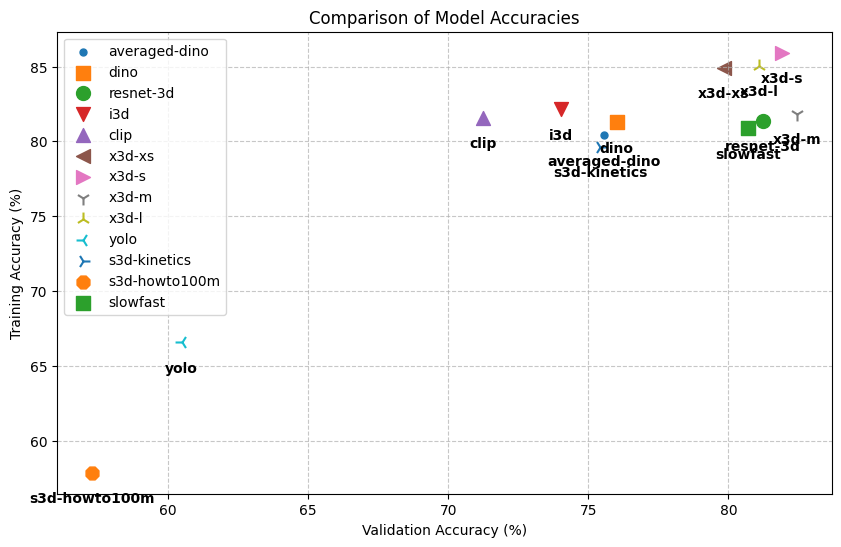
\includegraphics[width=0.475\textwidth]{assets/figures/models-scores.png}
    \caption{Your figure caption here.}
    \label{figure:models-performances}
\end{figure}

\begin{table}[h]
    \centering
    \tiny
    \begin{tabular}{|l|c|c|c|c|}
    \hline
    \textbf{Backbone} & \textbf{Accuracy} & \textbf{Edit Score} & \textbf{F1 Score} & \textbf{\# Parameters} \\
    \hline
    ResNet50          & 95 ± 0.1\%              & 92 ± 0.1\%                & 94 ± 0.1\%              & 25M                   \\
    VGG16             & 93 ± 0.1\%              & 90 ± 0.1\%                & 92 ± 0.1\%              & 138M                  \\
    InceptionV3       & 96 ± 0.1\%              & 94 ± 0.1\%                & 95 ± 0.1\%              & 23M                   \\
    EfficientNetB0    & 97 ± 0.1\%              & 95 ± 0.1\%                & 96 ± 0.1\%              & 5.3M                  \\
    $\cdots$            & $\cdots$                  & $\cdots$                    & $\cdots$                  & $\cdots$                \\
    Kinetics-SotA     & 95 \%                   & 95 \%                     & 95 \%                   & NA                    \\
    \hline
    \end{tabular}
    \caption{Model Performance Comparison}
    \label{table:models-performances}
\end{table}

\todo[inline]{Add a training time or number of epochs column in the table.}
\todo[inline]{Add a column to say whether the backbone is temporal or frame by frame.}
\todo[inline]{Add a column for the vision / temporal window, like how much frames are considered at once.}
\todo[inline]{Add a table that displays the per-class accuracy.}

From \ref{figure:models-performances} we can clearly see two backbone models underperforming compared to the other. First one is YOLO which is basically used to extract the key points estimation of the climber's skeleton, this keypoints are either concatenated or averaged to form the final features that are fed into the linear classifier, the underperformance of these features can be justified by the fact that the climbers can be moving while observing or brushing the holds, and they are also moving while climbing and the dynamic \& speed of the movement of the climber is very similar during the 3 actions, thus making it hard for the model to predict the class given this features. A possible improvement would be to take the absolute keypoints rather than the ones relative to the climber's center of mass, this would enable the model to distinguich between the different classes using the climber's position (if close to the wall then brushing, if above then climbing and if far then observing) but this would bias the model too much as a simple change in the camera position would give completely wrong predictions. 

The second under performing model is the S3D model trained on the HowTo100M dataset, as said in the \ref{subsection:popular-video-datasets}, the HowTo100M contains mostly instructional videos and thus the kind of interactions, movements and actions that are learned by the model are fine grained and detailed one, this makes the model very suited to capture very precise and fine grained actions but fails to capture big actions and movements such as in our case.
And this explanation can be confirmed as the same model but trained on a different dataset (Kinetics Dataset) that is more focused n big movements / actions rather than fine grained one gives considerably better results.
This demonstrate the important of the pre-training dataset.

We can also see a clear pattern which is that models that consider the temporal axis and work on clip / segment level for feature extraction performs better than the models based on frame level features, in both averaging the features on the frames or taking them as a whole.

We can also see that given our dataset size, using a larger model (x3d-m) don't necessarily yeilds better performances and even make them fall a little bit compared to smaller models (x3d-s).

We can also see that regarding frame based feature extractor, averaging the features, concatenating them or even performing temporal modeling on them using an LSTM don't yeild any improvement, this can be due to the dataset size as in some related work [\cite{example-paper-doing-temporal-modeling}, \cite{example-paper-doing-temporal-modeling}, \cite{example-paper-doing-temporal-modeling}] this step yeilds a significatif improvement in the model's performance.

Finalize by talking about the performance of each model and which one we should choose based on the requirements (if we need accuracy on a specific class, speed and inference time, model size, etc).

\todo[inline]{Maybe put this in the appendix for all the models and here display only one example, the best one.}
\todo[inline]{Show an illustration / example of segmentation and statistics of different models.}